
% Default to the notebook output style

    


% Inherit from the specified cell style.




    
\documentclass[11pt]{article}

    
    
    \usepackage[T1]{fontenc}
    % Nicer default font (+ math font) than Computer Modern for most use cases
    \usepackage{mathpazo}

    % Basic figure setup, for now with no caption control since it's done
    % automatically by Pandoc (which extracts ![](path) syntax from Markdown).
    \usepackage{graphicx}
    % We will generate all images so they have a width \maxwidth. This means
    % that they will get their normal width if they fit onto the page, but
    % are scaled down if they would overflow the margins.
    \makeatletter
    \def\maxwidth{\ifdim\Gin@nat@width>\linewidth\linewidth
    \else\Gin@nat@width\fi}
    \makeatother
    \let\Oldincludegraphics\includegraphics
    % Set max figure width to be 80% of text width, for now hardcoded.
    \renewcommand{\includegraphics}[1]{\Oldincludegraphics[width=.8\maxwidth]{#1}}
    % Ensure that by default, figures have no caption (until we provide a
    % proper Figure object with a Caption API and a way to capture that
    % in the conversion process - todo).
    \usepackage{caption}
    \DeclareCaptionLabelFormat{nolabel}{}
    \captionsetup{labelformat=nolabel}

    \usepackage{adjustbox} % Used to constrain images to a maximum size 
    \usepackage{xcolor} % Allow colors to be defined
    \usepackage{enumerate} % Needed for markdown enumerations to work
    \usepackage{geometry} % Used to adjust the document margins
    \usepackage{amsmath} % Equations
    \usepackage{amssymb} % Equations
    \usepackage{textcomp} % defines textquotesingle
    % Hack from http://tex.stackexchange.com/a/47451/13684:
    \AtBeginDocument{%
        \def\PYZsq{\textquotesingle}% Upright quotes in Pygmentized code
    }
    \usepackage{upquote} % Upright quotes for verbatim code
    \usepackage{eurosym} % defines \euro
    \usepackage[mathletters]{ucs} % Extended unicode (utf-8) support
    \usepackage[utf8x]{inputenc} % Allow utf-8 characters in the tex document
    \usepackage{fancyvrb} % verbatim replacement that allows latex
    \usepackage{grffile} % extends the file name processing of package graphics 
                         % to support a larger range 
    % The hyperref package gives us a pdf with properly built
    % internal navigation ('pdf bookmarks' for the table of contents,
    % internal cross-reference links, web links for URLs, etc.)
    \usepackage{hyperref}
    \usepackage{longtable} % longtable support required by pandoc >1.10
    \usepackage{booktabs}  % table support for pandoc > 1.12.2
    \usepackage[inline]{enumitem} % IRkernel/repr support (it uses the enumerate* environment)
    \usepackage[normalem]{ulem} % ulem is needed to support strikethroughs (\sout)
                                % normalem makes italics be italics, not underlines
    

    
    
    % Colors for the hyperref package
    \definecolor{urlcolor}{rgb}{0,.145,.698}
    \definecolor{linkcolor}{rgb}{.71,0.21,0.01}
    \definecolor{citecolor}{rgb}{.12,.54,.11}

    % ANSI colors
    \definecolor{ansi-black}{HTML}{3E424D}
    \definecolor{ansi-black-intense}{HTML}{282C36}
    \definecolor{ansi-red}{HTML}{E75C58}
    \definecolor{ansi-red-intense}{HTML}{B22B31}
    \definecolor{ansi-green}{HTML}{00A250}
    \definecolor{ansi-green-intense}{HTML}{007427}
    \definecolor{ansi-yellow}{HTML}{DDB62B}
    \definecolor{ansi-yellow-intense}{HTML}{B27D12}
    \definecolor{ansi-blue}{HTML}{208FFB}
    \definecolor{ansi-blue-intense}{HTML}{0065CA}
    \definecolor{ansi-magenta}{HTML}{D160C4}
    \definecolor{ansi-magenta-intense}{HTML}{A03196}
    \definecolor{ansi-cyan}{HTML}{60C6C8}
    \definecolor{ansi-cyan-intense}{HTML}{258F8F}
    \definecolor{ansi-white}{HTML}{C5C1B4}
    \definecolor{ansi-white-intense}{HTML}{A1A6B2}

    % commands and environments needed by pandoc snippets
    % extracted from the output of `pandoc -s`
    \providecommand{\tightlist}{%
      \setlength{\itemsep}{0pt}\setlength{\parskip}{0pt}}
    \DefineVerbatimEnvironment{Highlighting}{Verbatim}{commandchars=\\\{\}}
    % Add ',fontsize=\small' for more characters per line
    \newenvironment{Shaded}{}{}
    \newcommand{\KeywordTok}[1]{\textcolor[rgb]{0.00,0.44,0.13}{\textbf{{#1}}}}
    \newcommand{\DataTypeTok}[1]{\textcolor[rgb]{0.56,0.13,0.00}{{#1}}}
    \newcommand{\DecValTok}[1]{\textcolor[rgb]{0.25,0.63,0.44}{{#1}}}
    \newcommand{\BaseNTok}[1]{\textcolor[rgb]{0.25,0.63,0.44}{{#1}}}
    \newcommand{\FloatTok}[1]{\textcolor[rgb]{0.25,0.63,0.44}{{#1}}}
    \newcommand{\CharTok}[1]{\textcolor[rgb]{0.25,0.44,0.63}{{#1}}}
    \newcommand{\StringTok}[1]{\textcolor[rgb]{0.25,0.44,0.63}{{#1}}}
    \newcommand{\CommentTok}[1]{\textcolor[rgb]{0.38,0.63,0.69}{\textit{{#1}}}}
    \newcommand{\OtherTok}[1]{\textcolor[rgb]{0.00,0.44,0.13}{{#1}}}
    \newcommand{\AlertTok}[1]{\textcolor[rgb]{1.00,0.00,0.00}{\textbf{{#1}}}}
    \newcommand{\FunctionTok}[1]{\textcolor[rgb]{0.02,0.16,0.49}{{#1}}}
    \newcommand{\RegionMarkerTok}[1]{{#1}}
    \newcommand{\ErrorTok}[1]{\textcolor[rgb]{1.00,0.00,0.00}{\textbf{{#1}}}}
    \newcommand{\NormalTok}[1]{{#1}}
    
    % Additional commands for more recent versions of Pandoc
    \newcommand{\ConstantTok}[1]{\textcolor[rgb]{0.53,0.00,0.00}{{#1}}}
    \newcommand{\SpecialCharTok}[1]{\textcolor[rgb]{0.25,0.44,0.63}{{#1}}}
    \newcommand{\VerbatimStringTok}[1]{\textcolor[rgb]{0.25,0.44,0.63}{{#1}}}
    \newcommand{\SpecialStringTok}[1]{\textcolor[rgb]{0.73,0.40,0.53}{{#1}}}
    \newcommand{\ImportTok}[1]{{#1}}
    \newcommand{\DocumentationTok}[1]{\textcolor[rgb]{0.73,0.13,0.13}{\textit{{#1}}}}
    \newcommand{\AnnotationTok}[1]{\textcolor[rgb]{0.38,0.63,0.69}{\textbf{\textit{{#1}}}}}
    \newcommand{\CommentVarTok}[1]{\textcolor[rgb]{0.38,0.63,0.69}{\textbf{\textit{{#1}}}}}
    \newcommand{\VariableTok}[1]{\textcolor[rgb]{0.10,0.09,0.49}{{#1}}}
    \newcommand{\ControlFlowTok}[1]{\textcolor[rgb]{0.00,0.44,0.13}{\textbf{{#1}}}}
    \newcommand{\OperatorTok}[1]{\textcolor[rgb]{0.40,0.40,0.40}{{#1}}}
    \newcommand{\BuiltInTok}[1]{{#1}}
    \newcommand{\ExtensionTok}[1]{{#1}}
    \newcommand{\PreprocessorTok}[1]{\textcolor[rgb]{0.74,0.48,0.00}{{#1}}}
    \newcommand{\AttributeTok}[1]{\textcolor[rgb]{0.49,0.56,0.16}{{#1}}}
    \newcommand{\InformationTok}[1]{\textcolor[rgb]{0.38,0.63,0.69}{\textbf{\textit{{#1}}}}}
    \newcommand{\WarningTok}[1]{\textcolor[rgb]{0.38,0.63,0.69}{\textbf{\textit{{#1}}}}}
    
    
    % Define a nice break command that doesn't care if a line doesn't already
    % exist.
    \def\br{\hspace*{\fill} \\* }
    % Math Jax compatability definitions
    \def\gt{>}
    \def\lt{<}
    % Document parameters
    \title{RL-Quadcopter}
    
    
    

    % Pygments definitions
    
\makeatletter
\def\PY@reset{\let\PY@it=\relax \let\PY@bf=\relax%
    \let\PY@ul=\relax \let\PY@tc=\relax%
    \let\PY@bc=\relax \let\PY@ff=\relax}
\def\PY@tok#1{\csname PY@tok@#1\endcsname}
\def\PY@toks#1+{\ifx\relax#1\empty\else%
    \PY@tok{#1}\expandafter\PY@toks\fi}
\def\PY@do#1{\PY@bc{\PY@tc{\PY@ul{%
    \PY@it{\PY@bf{\PY@ff{#1}}}}}}}
\def\PY#1#2{\PY@reset\PY@toks#1+\relax+\PY@do{#2}}

\expandafter\def\csname PY@tok@gd\endcsname{\def\PY@tc##1{\textcolor[rgb]{0.63,0.00,0.00}{##1}}}
\expandafter\def\csname PY@tok@gu\endcsname{\let\PY@bf=\textbf\def\PY@tc##1{\textcolor[rgb]{0.50,0.00,0.50}{##1}}}
\expandafter\def\csname PY@tok@gt\endcsname{\def\PY@tc##1{\textcolor[rgb]{0.00,0.27,0.87}{##1}}}
\expandafter\def\csname PY@tok@gs\endcsname{\let\PY@bf=\textbf}
\expandafter\def\csname PY@tok@gr\endcsname{\def\PY@tc##1{\textcolor[rgb]{1.00,0.00,0.00}{##1}}}
\expandafter\def\csname PY@tok@cm\endcsname{\let\PY@it=\textit\def\PY@tc##1{\textcolor[rgb]{0.25,0.50,0.50}{##1}}}
\expandafter\def\csname PY@tok@vg\endcsname{\def\PY@tc##1{\textcolor[rgb]{0.10,0.09,0.49}{##1}}}
\expandafter\def\csname PY@tok@vi\endcsname{\def\PY@tc##1{\textcolor[rgb]{0.10,0.09,0.49}{##1}}}
\expandafter\def\csname PY@tok@vm\endcsname{\def\PY@tc##1{\textcolor[rgb]{0.10,0.09,0.49}{##1}}}
\expandafter\def\csname PY@tok@mh\endcsname{\def\PY@tc##1{\textcolor[rgb]{0.40,0.40,0.40}{##1}}}
\expandafter\def\csname PY@tok@cs\endcsname{\let\PY@it=\textit\def\PY@tc##1{\textcolor[rgb]{0.25,0.50,0.50}{##1}}}
\expandafter\def\csname PY@tok@ge\endcsname{\let\PY@it=\textit}
\expandafter\def\csname PY@tok@vc\endcsname{\def\PY@tc##1{\textcolor[rgb]{0.10,0.09,0.49}{##1}}}
\expandafter\def\csname PY@tok@il\endcsname{\def\PY@tc##1{\textcolor[rgb]{0.40,0.40,0.40}{##1}}}
\expandafter\def\csname PY@tok@go\endcsname{\def\PY@tc##1{\textcolor[rgb]{0.53,0.53,0.53}{##1}}}
\expandafter\def\csname PY@tok@cp\endcsname{\def\PY@tc##1{\textcolor[rgb]{0.74,0.48,0.00}{##1}}}
\expandafter\def\csname PY@tok@gi\endcsname{\def\PY@tc##1{\textcolor[rgb]{0.00,0.63,0.00}{##1}}}
\expandafter\def\csname PY@tok@gh\endcsname{\let\PY@bf=\textbf\def\PY@tc##1{\textcolor[rgb]{0.00,0.00,0.50}{##1}}}
\expandafter\def\csname PY@tok@ni\endcsname{\let\PY@bf=\textbf\def\PY@tc##1{\textcolor[rgb]{0.60,0.60,0.60}{##1}}}
\expandafter\def\csname PY@tok@nl\endcsname{\def\PY@tc##1{\textcolor[rgb]{0.63,0.63,0.00}{##1}}}
\expandafter\def\csname PY@tok@nn\endcsname{\let\PY@bf=\textbf\def\PY@tc##1{\textcolor[rgb]{0.00,0.00,1.00}{##1}}}
\expandafter\def\csname PY@tok@no\endcsname{\def\PY@tc##1{\textcolor[rgb]{0.53,0.00,0.00}{##1}}}
\expandafter\def\csname PY@tok@na\endcsname{\def\PY@tc##1{\textcolor[rgb]{0.49,0.56,0.16}{##1}}}
\expandafter\def\csname PY@tok@nb\endcsname{\def\PY@tc##1{\textcolor[rgb]{0.00,0.50,0.00}{##1}}}
\expandafter\def\csname PY@tok@nc\endcsname{\let\PY@bf=\textbf\def\PY@tc##1{\textcolor[rgb]{0.00,0.00,1.00}{##1}}}
\expandafter\def\csname PY@tok@nd\endcsname{\def\PY@tc##1{\textcolor[rgb]{0.67,0.13,1.00}{##1}}}
\expandafter\def\csname PY@tok@ne\endcsname{\let\PY@bf=\textbf\def\PY@tc##1{\textcolor[rgb]{0.82,0.25,0.23}{##1}}}
\expandafter\def\csname PY@tok@nf\endcsname{\def\PY@tc##1{\textcolor[rgb]{0.00,0.00,1.00}{##1}}}
\expandafter\def\csname PY@tok@si\endcsname{\let\PY@bf=\textbf\def\PY@tc##1{\textcolor[rgb]{0.73,0.40,0.53}{##1}}}
\expandafter\def\csname PY@tok@s2\endcsname{\def\PY@tc##1{\textcolor[rgb]{0.73,0.13,0.13}{##1}}}
\expandafter\def\csname PY@tok@nt\endcsname{\let\PY@bf=\textbf\def\PY@tc##1{\textcolor[rgb]{0.00,0.50,0.00}{##1}}}
\expandafter\def\csname PY@tok@nv\endcsname{\def\PY@tc##1{\textcolor[rgb]{0.10,0.09,0.49}{##1}}}
\expandafter\def\csname PY@tok@s1\endcsname{\def\PY@tc##1{\textcolor[rgb]{0.73,0.13,0.13}{##1}}}
\expandafter\def\csname PY@tok@dl\endcsname{\def\PY@tc##1{\textcolor[rgb]{0.73,0.13,0.13}{##1}}}
\expandafter\def\csname PY@tok@ch\endcsname{\let\PY@it=\textit\def\PY@tc##1{\textcolor[rgb]{0.25,0.50,0.50}{##1}}}
\expandafter\def\csname PY@tok@m\endcsname{\def\PY@tc##1{\textcolor[rgb]{0.40,0.40,0.40}{##1}}}
\expandafter\def\csname PY@tok@gp\endcsname{\let\PY@bf=\textbf\def\PY@tc##1{\textcolor[rgb]{0.00,0.00,0.50}{##1}}}
\expandafter\def\csname PY@tok@sh\endcsname{\def\PY@tc##1{\textcolor[rgb]{0.73,0.13,0.13}{##1}}}
\expandafter\def\csname PY@tok@ow\endcsname{\let\PY@bf=\textbf\def\PY@tc##1{\textcolor[rgb]{0.67,0.13,1.00}{##1}}}
\expandafter\def\csname PY@tok@sx\endcsname{\def\PY@tc##1{\textcolor[rgb]{0.00,0.50,0.00}{##1}}}
\expandafter\def\csname PY@tok@bp\endcsname{\def\PY@tc##1{\textcolor[rgb]{0.00,0.50,0.00}{##1}}}
\expandafter\def\csname PY@tok@c1\endcsname{\let\PY@it=\textit\def\PY@tc##1{\textcolor[rgb]{0.25,0.50,0.50}{##1}}}
\expandafter\def\csname PY@tok@fm\endcsname{\def\PY@tc##1{\textcolor[rgb]{0.00,0.00,1.00}{##1}}}
\expandafter\def\csname PY@tok@o\endcsname{\def\PY@tc##1{\textcolor[rgb]{0.40,0.40,0.40}{##1}}}
\expandafter\def\csname PY@tok@kc\endcsname{\let\PY@bf=\textbf\def\PY@tc##1{\textcolor[rgb]{0.00,0.50,0.00}{##1}}}
\expandafter\def\csname PY@tok@c\endcsname{\let\PY@it=\textit\def\PY@tc##1{\textcolor[rgb]{0.25,0.50,0.50}{##1}}}
\expandafter\def\csname PY@tok@mf\endcsname{\def\PY@tc##1{\textcolor[rgb]{0.40,0.40,0.40}{##1}}}
\expandafter\def\csname PY@tok@err\endcsname{\def\PY@bc##1{\setlength{\fboxsep}{0pt}\fcolorbox[rgb]{1.00,0.00,0.00}{1,1,1}{\strut ##1}}}
\expandafter\def\csname PY@tok@mb\endcsname{\def\PY@tc##1{\textcolor[rgb]{0.40,0.40,0.40}{##1}}}
\expandafter\def\csname PY@tok@ss\endcsname{\def\PY@tc##1{\textcolor[rgb]{0.10,0.09,0.49}{##1}}}
\expandafter\def\csname PY@tok@sr\endcsname{\def\PY@tc##1{\textcolor[rgb]{0.73,0.40,0.53}{##1}}}
\expandafter\def\csname PY@tok@mo\endcsname{\def\PY@tc##1{\textcolor[rgb]{0.40,0.40,0.40}{##1}}}
\expandafter\def\csname PY@tok@kd\endcsname{\let\PY@bf=\textbf\def\PY@tc##1{\textcolor[rgb]{0.00,0.50,0.00}{##1}}}
\expandafter\def\csname PY@tok@mi\endcsname{\def\PY@tc##1{\textcolor[rgb]{0.40,0.40,0.40}{##1}}}
\expandafter\def\csname PY@tok@kn\endcsname{\let\PY@bf=\textbf\def\PY@tc##1{\textcolor[rgb]{0.00,0.50,0.00}{##1}}}
\expandafter\def\csname PY@tok@cpf\endcsname{\let\PY@it=\textit\def\PY@tc##1{\textcolor[rgb]{0.25,0.50,0.50}{##1}}}
\expandafter\def\csname PY@tok@kr\endcsname{\let\PY@bf=\textbf\def\PY@tc##1{\textcolor[rgb]{0.00,0.50,0.00}{##1}}}
\expandafter\def\csname PY@tok@s\endcsname{\def\PY@tc##1{\textcolor[rgb]{0.73,0.13,0.13}{##1}}}
\expandafter\def\csname PY@tok@kp\endcsname{\def\PY@tc##1{\textcolor[rgb]{0.00,0.50,0.00}{##1}}}
\expandafter\def\csname PY@tok@w\endcsname{\def\PY@tc##1{\textcolor[rgb]{0.73,0.73,0.73}{##1}}}
\expandafter\def\csname PY@tok@kt\endcsname{\def\PY@tc##1{\textcolor[rgb]{0.69,0.00,0.25}{##1}}}
\expandafter\def\csname PY@tok@sc\endcsname{\def\PY@tc##1{\textcolor[rgb]{0.73,0.13,0.13}{##1}}}
\expandafter\def\csname PY@tok@sb\endcsname{\def\PY@tc##1{\textcolor[rgb]{0.73,0.13,0.13}{##1}}}
\expandafter\def\csname PY@tok@sa\endcsname{\def\PY@tc##1{\textcolor[rgb]{0.73,0.13,0.13}{##1}}}
\expandafter\def\csname PY@tok@k\endcsname{\let\PY@bf=\textbf\def\PY@tc##1{\textcolor[rgb]{0.00,0.50,0.00}{##1}}}
\expandafter\def\csname PY@tok@se\endcsname{\let\PY@bf=\textbf\def\PY@tc##1{\textcolor[rgb]{0.73,0.40,0.13}{##1}}}
\expandafter\def\csname PY@tok@sd\endcsname{\let\PY@it=\textit\def\PY@tc##1{\textcolor[rgb]{0.73,0.13,0.13}{##1}}}

\def\PYZbs{\char`\\}
\def\PYZus{\char`\_}
\def\PYZob{\char`\{}
\def\PYZcb{\char`\}}
\def\PYZca{\char`\^}
\def\PYZam{\char`\&}
\def\PYZlt{\char`\<}
\def\PYZgt{\char`\>}
\def\PYZsh{\char`\#}
\def\PYZpc{\char`\%}
\def\PYZdl{\char`\$}
\def\PYZhy{\char`\-}
\def\PYZsq{\char`\'}
\def\PYZdq{\char`\"}
\def\PYZti{\char`\~}
% for compatibility with earlier versions
\def\PYZat{@}
\def\PYZlb{[}
\def\PYZrb{]}
\makeatother


    % Exact colors from NB
    \definecolor{incolor}{rgb}{0.0, 0.0, 0.5}
    \definecolor{outcolor}{rgb}{0.545, 0.0, 0.0}



    
    % Prevent overflowing lines due to hard-to-break entities
    \sloppy 
    % Setup hyperref package
    \hypersetup{
      breaklinks=true,  % so long urls are correctly broken across lines
      colorlinks=true,
      urlcolor=urlcolor,
      linkcolor=linkcolor,
      citecolor=citecolor,
      }
    % Slightly bigger margins than the latex defaults
    
    \geometry{verbose,tmargin=1in,bmargin=1in,lmargin=1in,rmargin=1in}
    
    

    \begin{document}
    
    
    \maketitle
    
    

    
    \hypertarget{project-train-a-quadcopter-how-to-fly}{%
\section{Project: Train a Quadcopter How to
Fly}\label{project-train-a-quadcopter-how-to-fly}}

Design an agent that can fly a quadcopter, and then train it using a
reinforcement learning algorithm of your choice! Try to apply the
techniques you have learnt, but also feel free to come up with
innovative ideas and test them.

\begin{figure}
\centering
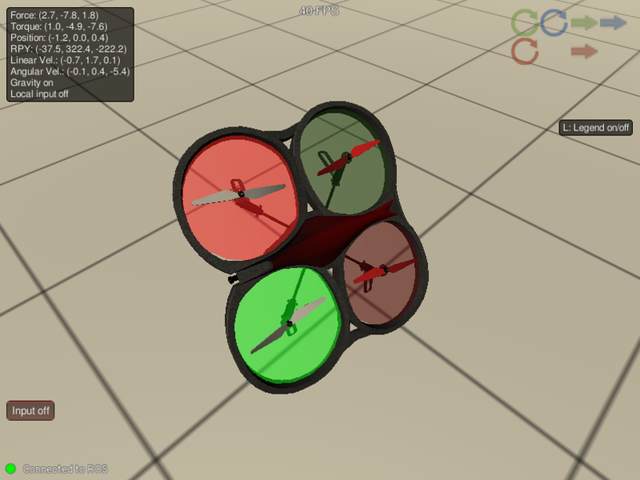
\includegraphics{images/quadcopter_tumble.png}
\caption{Quadcopter doing a flip trying to takeoff from the ground}
\end{figure}

\hypertarget{instructions}{%
\subsection{Instructions}\label{instructions}}

\begin{quote}
\textbf{Note}: If you haven't done so already, follow the steps in this
repo's README to install ROS, and ensure that the simulator is running
and correctly connecting to ROS.
\end{quote}

When you are ready to start coding, take a look at the
\texttt{quad\_controller\_rl/src/} (source) directory to better
understand the structure. Here are some of the salient items:

\begin{itemize}
\tightlist
\item
  \texttt{src/}: Contains all the source code for the project.

  \begin{itemize}
  \tightlist
  \item
    \texttt{quad\_controller\_rl/}: This is the root of the Python
    package you'll be working in.
  \item
    \ldots{}
  \item
    \texttt{tasks/}: Define your tasks (environments) in this
    sub-directory.

    \begin{itemize}
    \tightlist
    \item
      \texttt{\_\_init\_\_.py}: When you define a new task, you'll have
      to import it here.
    \item
      \texttt{base\_task.py}: Generic base class for all tasks, with
      documentation.
    \item
      \texttt{takeoff.py}: This is the first task, already defined for
      you, and set to run by default.
    \end{itemize}
  \item
    \ldots{}
  \item
    \texttt{agents/}: Develop your reinforcement learning agents here.

    \begin{itemize}
    \tightlist
    \item
      \texttt{\_\_init\_\_.py}: When you define a new agent, you'll have
      to import it here, just like tasks.
    \item
      \texttt{base\_agent.py}: Generic base class for all agents, with
      documentation.
    \item
      \texttt{policy\_search.py}: A sample agent has been provided here,
      and is set to run by default.
    \end{itemize}
  \item
    \ldots{}
  \end{itemize}
\end{itemize}

\hypertarget{tasks}{%
\subsubsection{Tasks}\label{tasks}}

Open up the base class for tasks, \texttt{BaseTask}, defined in
\texttt{tasks/base\_task.py}:

\begin{Shaded}
\begin{Highlighting}[]
\KeywordTok{class}\NormalTok{ BaseTask:}
    \CommentTok{"""Generic base class for reinforcement learning tasks."""}

    \KeywordTok{def} \FunctionTok{__init__}\NormalTok{(}\VariableTok{self}\NormalTok{):}
        \CommentTok{"""Define state and action spaces, initialize other task parameters."""}
        \ControlFlowTok{pass}
    
    \KeywordTok{def}\NormalTok{ set_agent(}\VariableTok{self}\NormalTok{, agent):}
        \CommentTok{"""Set an agent to carry out this task; to be called from update."""}
        \VariableTok{self}\NormalTok{.agent }\OperatorTok{=}\NormalTok{ agent}
    
    \KeywordTok{def}\NormalTok{ reset(}\VariableTok{self}\NormalTok{):}
        \CommentTok{"""Reset task and return initial condition."""}
        \ControlFlowTok{raise} \PreprocessorTok{NotImplementedError}
    
    \KeywordTok{def}\NormalTok{ update(}\VariableTok{self}\NormalTok{, timestamp, pose, angular_velocity, linear_acceleration):}
        \CommentTok{"""Process current data, call agent, return action and done flag."""}
        \ControlFlowTok{raise} \PreprocessorTok{NotImplementedError}            
\end{Highlighting}
\end{Shaded}

All tasks must inherit from this class to function properly. You will
need to override the \texttt{reset()} and \texttt{update()} methods when
defining a task, otherwise you will get \texttt{NotImplementedError}'s.
Besides these two, you should define the state (observation) space and
the action space for the task in the constructor,
\texttt{\_\_init\_\_()}, and initialize any other variables you may need
to run the task.

Now compare this with the first concrete task \texttt{Takeoff}, defined
in \texttt{tasks/takeoff.py}:

\begin{Shaded}
\begin{Highlighting}[]
\KeywordTok{class}\NormalTok{ Takeoff(BaseTask):}
    \CommentTok{"""Simple task where the goal is to lift off the ground and reach a target height."""}
\NormalTok{    ...}
\end{Highlighting}
\end{Shaded}

In \texttt{\_\_init\_\_()}, notice how the state and action spaces are
defined using \href{https://gym.openai.com/docs/\#spaces}{OpenAI Gym
spaces}, like
\href{https://github.com/openai/gym/blob/master/gym/spaces/box.py}{\texttt{Box}}.
These objects provide a clean and powerful interface for agents to
explore. For instance, they can inspect the dimensionality of a space
(\texttt{shape}), ask for the limits (\texttt{high} and \texttt{low}),
or even sample a bunch of observations using the \texttt{sample()}
method, before beginning to interact with the environment. We also set a
time limit (\texttt{max\_duration}) for each episode here, and the
height (\texttt{target\_z}) that the quadcopter needs to reach for a
successful takeoff.

The \texttt{reset()} method is meant to give you a chance to
reset/initialize any variables you need in order to prepare for the next
episode. You do not need to call it yourself; it will be invoked
externally. And yes, it will be called once before each episode,
including the very first one. Here \texttt{Takeoff} doesn't have any
episode variables to initialize, but it must return a valid
\emph{initial condition} for the task, which is a tuple consisting of a
\href{http://docs.ros.org/api/geometry_msgs/html/msg/Pose.html}{\texttt{Pose}}
and
\href{http://docs.ros.org/api/geometry_msgs/html/msg/Twist.html}{\texttt{Twist}}
object. These are ROS message types used to convey the pose (position,
orientation) and velocity (linear, angular) you want the quadcopter to
have at the beginning of an episode. You may choose to supply the same
initial values every time, or change it a little bit, e.g.
\texttt{Takeoff} drops the quadcopter off from a small height with a bit
of randomness.

\begin{quote}
\textbf{Tip}: Slightly randomized initial conditions can help the agent
explore the state space faster.
\end{quote}

Finally, the \texttt{update()} method is perhaps the most important.
This is where you define the dynamics of the task and engage the agent.
It is called by a ROS process periodically (roughly 30 times a second,
by default), with current data from the simulation. A number of
arguments are available: \texttt{timestamp} (you can use this to check
for timeout, or compute velocities), \texttt{pose} (position,
orientation of the quadcopter), \texttt{angular\_velocity}, and
\texttt{linear\_acceleration}. You do not have to include all these
variables in every task, e.g. \texttt{Takeoff} only uses pose
information, and even that requires a 7-element state vector.

Once you have prepared the state you want to pass on to your agent, you
will need to compute the reward, and check whether the episode is
complete (e.g.~agent crossed the time limit, or reached a certain
height). Note that these two things (\texttt{reward} and \texttt{done})
are based on actions that the agent took in the past. When you are
writing your own agents, you have to be mindful of this.

Now you can pass in the \texttt{state}, \texttt{reward} and
\texttt{done} values to the agent's \texttt{step()} method and expect an
action vector back that matches the action space that you have defined,
in this case a \texttt{Box(6,)}. After checking that the action vector
is non-empty, and clamping it to the space limits, you have to convert
it into a ROS \texttt{Wrench} message. The first 3 elements of the
action vector are interpreted as force in x, y, z directions, and the
remaining 3 elements convey the torque to be applied around those axes,
respectively.

Return the \texttt{Wrench} object (or \texttt{None} if you don't want to
take any action) and the \texttt{done} flag from your \texttt{update()}
method (note that when \texttt{done} is \texttt{True}, the
\texttt{Wrench} object is ignored, so you can return \texttt{None}
instead). This will be passed back to the simulation as a control
command, and will affect the quadcopter's pose, orientation, velocity,
etc. You will be able to gauge the effect when the \texttt{update()}
method is called in the next time step.

\hypertarget{agents}{%
\subsubsection{Agents}\label{agents}}

Reinforcement learning agents are defined in a similar way. Open up the
generic agent class, \texttt{BaseAgent}, defined in
\texttt{agents/base\_agent.py}, and the sample agent
\texttt{RandomPolicySearch} defined in
\texttt{agents/policy\_search.py}. They are actually even simpler to
define - you only need to implement the \texttt{step()} method that is
discussed above. It needs to consume \texttt{state} (vector),
\texttt{reward} (scalar value) and \texttt{done} (boolean), and produce
an \texttt{action} (vector). The state and action vectors must match the
respective space indicated by the task. And that's it!

Well, that's just to get things working correctly! The sample agent
given \texttt{RandomPolicySearch} uses a very simplistic linear policy
to directly compute the action vector as a dot product of the state
vector and a matrix of weights. Then, it randomly perturbs the
parameters by adding some Gaussian noise, to produce a different policy.
Based on the average reward obtained in each episode (``score''), it
keeps track of the best set of parameters found so far, how the score is
changing, and accordingly tweaks a scaling factor to widen or tighten
the noise.

    \begin{Verbatim}[commandchars=\\\{\}]
{\color{incolor}In [{\color{incolor}1}]:} \PY{o}{\PYZpc{}\PYZpc{}}\PY{k}{html}
        \PYZlt{}div style=\PYZdq{}width: 100\PYZpc{}; text\PYZhy{}align: center;\PYZdq{}\PYZgt{}
            \PYZlt{}h3\PYZgt{}Teach a Quadcopter How to Tumble\PYZlt{}/h3\PYZgt{}
            \PYZlt{}video poster=\PYZdq{}images/quadcopter\PYZus{}tumble.png\PYZdq{} width=\PYZdq{}640\PYZdq{} controls muted\PYZgt{}
                \PYZlt{}source src=\PYZdq{}images/quadcopter\PYZus{}tumble.mp4\PYZdq{} type=\PYZdq{}video/mp4\PYZdq{} /\PYZgt{}
                \PYZlt{}p\PYZgt{}Video: Quadcopter tumbling, trying to get off the ground\PYZlt{}/p\PYZgt{}
            \PYZlt{}/video\PYZgt{}
        \PYZlt{}/div\PYZgt{}
\end{Verbatim}


    
    \begin{verbatim}
<IPython.core.display.HTML object>
    \end{verbatim}

    
    Obviously, this agent performs very poorly on the task. It does manage
to move the quadcopter, which is good, but instead of a stable takeoff,
it often leads to dizzying cartwheels and somersaults! And that's where
you come in - your first \emph{task} is to design a better agent for
this takeoff task. Instead of messing with the sample agent, create new
file in the \texttt{agents/} directory, say
\texttt{policy\_gradients.py}, and define your own agent in it. Remember
to inherit from the base agent class, e.g.:

\begin{Shaded}
\begin{Highlighting}[]
\KeywordTok{class}\NormalTok{ DDPG(BaseAgent):}
\NormalTok{    ...}
\end{Highlighting}
\end{Shaded}

You can borrow whatever you need from the sample agent, including ideas
on how you might modularize your code (using helper methods like
\texttt{act()}, \texttt{learn()}, \texttt{reset\_episode\_vars()},
etc.).

\begin{quote}
\textbf{Note}: This setup may look similar to the common OpenAI Gym
paradigm, but there is one small yet important difference. Instead of
the agent calling a method on the environment (to execute an action and
obtain the resulting state, reward and done value), here it is the task
that is calling a method on the agent (\texttt{step()}). If you plan to
store experience tuples for learning, you will need to cache the last
state (\(S_{t-1}\)) and last action taken (\(A_{t-1}\)), then in the
next time step when you get the new state (\(S_t\)) and reward
(\(R_t\)), you can store them along with the \texttt{done} flag
(\(\left\langle S_{t-1}, A_{t-1}, R_t, S_t, \mathrm{done?}\right\rangle\)).
\end{quote}

When an episode ends, the agent receives one last call to the
\texttt{step()} method with \texttt{done} set to \texttt{True} - this is
your chance to perform any cleanup/reset/batch-learning (note that no
reset method is called on an agent externally). The action returned on
this last call is ignored, so you may safely return \texttt{None}. The
next call would be the beginning of a new episode.

One last thing - in order to run your agent, you will have to edit
\texttt{agents/\_\_init\_\_.py} and import your agent class in it, e.g.:

\begin{Shaded}
\begin{Highlighting}[]
\ImportTok{from}\NormalTok{ quad_controller_rl.agents.policy_gradients }\ImportTok{import}\NormalTok{ DDPG}
\end{Highlighting}
\end{Shaded}

Then, while launching ROS, you will need to specify this class name on
the commandline/terminal:

\begin{Shaded}
\begin{Highlighting}[]
\ExtensionTok{roslaunch}\NormalTok{ quad_controller_rl rl_controller.launch agent:=DDPG}
\end{Highlighting}
\end{Shaded}

Okay, now the first task is cut out for you - follow the instructions
below to implement an agent that learns to take off from the ground. For
the remaining tasks, you get to define the tasks as well as the agents!
Use the \texttt{Takeoff} task as a guide, and refer to the
\texttt{BaseTask} docstrings for the different methods you need to
override. Use some debug print statements to understand the flow of
control better. And just like creating new agents, new tasks must
inherit \texttt{BaseTask}, they need be imported into
\texttt{tasks/\_\_init\_\_.py}, and specified on the commandline when
running:

\begin{Shaded}
\begin{Highlighting}[]
\ExtensionTok{roslaunch}\NormalTok{ quad_controller_rl rl_controller.launch task:=Hover agent:=DDPG}
\end{Highlighting}
\end{Shaded}

\begin{quote}
\textbf{Tip}: You typically need to launch ROS and then run the
simulator manually. But you can automate that process by either
copying/symlinking your simulator to
\texttt{quad\_controller\_rl/sim/DroneSim} (\texttt{DroneSim} must be an
executable/link to one), or by specifying it on the command line, as
follows:

\begin{Shaded}
\begin{Highlighting}[]
\ExtensionTok{roslaunch}\NormalTok{ quad_controller_rl rl_controller.launch task:=Hover agent:=DDPG sim:=}\OperatorTok{<}\NormalTok{full path}\OperatorTok{>}
\end{Highlighting}
\end{Shaded}
\end{quote}

\hypertarget{task-1-takeoff}{%
\subsection{Task 1: Takeoff}\label{task-1-takeoff}}

\hypertarget{implement-takeoff-agent}{%
\subsubsection{Implement takeoff agent}\label{implement-takeoff-agent}}

Train an agent to successfully lift off from the ground and reach a
certain threshold height. Develop your agent in a file under
\texttt{agents/} as described above, implementing at least the
\texttt{step()} method, and any other supporting methods that might be
necessary. You may use any reinforcement learning algorithm of your
choice (note that the action space consists of continuous variables, so
that may somewhat limit your choices).

The task has already been defined (in \texttt{tasks/takeoff.py}), which
you should not edit. The default target height (Z-axis value) to reach
is 10 units above the ground. And the reward function is essentially the
negative absolute distance from that set point (upto some threshold). An
episode ends when the quadcopter reaches the target height (x and y
values, orientation, velocity, etc. are ignored), or when the maximum
duration is crossed (5 seconds). See \texttt{Takeoff.update()} for more
details, including episode bonus/penalty.

As you develop your agent, it's important to keep an eye on how it's
performing. Build in a mechanism to log/save the total rewards obtained
in each episode to file. Once you are satisfied with your agent's
performance, return to this notebook to plot episode rewards, and answer
the questions below.

\hypertarget{plot-episode-rewards}{%
\subsubsection{Plot episode rewards}\label{plot-episode-rewards}}

Plot the total rewards obtained in each episode, either from a single
run, or averaged over multiple runs.
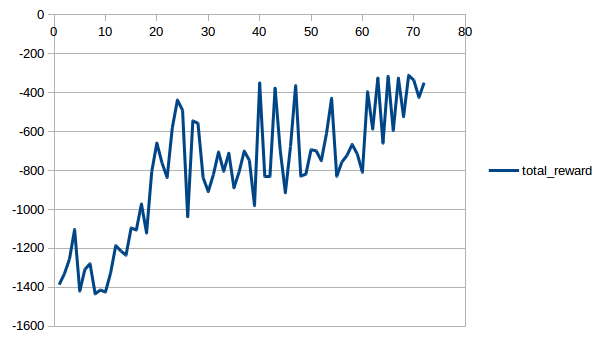
\includegraphics{images/takeoff.png}

    \textbf{Q}: What algorithm did you use? Briefly discuss why you chose it
for this task.

\textbf{A}: I used Continuous control with deep reinforcement
learning(DDPG) algorithm to train the quadcopter. It is a generalized
algorithm whick can be used in any domain.It can be applied into the
continuous domain and uses neural network for training which improves
the perfomance of the system.

\textbf{Q}: Using the episode rewards plot, discuss how the agent
learned over time.

\textbf{A}: - It was a gradual learning, after 20 episodes it started
flying(takeoff) to the max\_height. - The mean reward was around -400 at
last. - The learning was not too hard but the reward function was not
that good for the proper takoff, without jerks and toppling. - The
reward function was structured such that the there was incentive for
quadcopter to move up, but there was not any penality for the quadcopter
not to toggle/spin. The reward function should contain orientation term
to avoid toppling, rotatation of the quadcopter. As per the reward the
quadcopter has learned over time how to go up, after few episodes the
quadcopter achieves the maximum z-Force to go up, which is the optimal
policy.

\begin{itemize}
\item
  Just by looking at the problem domain for take off one can deduce that
  only z-force plays the part. Rest all the parameters are not
  significant. So one can always do - x-force = 0 y-force = 0 z-force =
  predict only this parameter by neural network. x-torque = 0 y-torque =
  0 z-torque = 0 Train the system for only predicting z-force.

  This the video when I trained the quadcopter for z-force only.
\end{itemize}

    \begin{Verbatim}[commandchars=\\\{\}]
{\color{incolor}In [{\color{incolor}3}]:} \PY{o}{\PYZpc{}\PYZpc{}}\PY{k}{html}
        \PYZlt{}div style=\PYZdq{}width: 100\PYZpc{}; text\PYZhy{}align: center;\PYZdq{}\PYZgt{}
            \PYZlt{}h3\PYZgt{}Quadcopter takeoff\PYZlt{}/h3\PYZgt{}
            \PYZlt{}video poster=\PYZdq{}images/image.png\PYZdq{} width=\PYZdq{}640\PYZdq{} controls muted\PYZgt{}
                \PYZlt{}source src=\PYZdq{}images/takeoff.mp4\PYZdq{} type=\PYZdq{}video/mp4\PYZdq{} /\PYZgt{}
                \PYZlt{}p\PYZgt{}Video: Quadcopter tumbling, trying to get off the ground\PYZlt{}/p\PYZgt{}
            \PYZlt{}/video\PYZgt{}
        \PYZlt{}/div\PYZgt{}
\end{Verbatim}


    
    \begin{verbatim}
<IPython.core.display.HTML object>
    \end{verbatim}

    
    \hypertarget{task-2-hover}{%
\subsection{Task 2: Hover}\label{task-2-hover}}

\hypertarget{implement-hover-agent}{%
\subsubsection{Implement hover agent}\label{implement-hover-agent}}

Now, your agent must take off and hover at the specified set point (say,
10 units above the ground). Same as before, you will need to create an
agent and implement the \texttt{step()} method (and any other supporting
methods) to apply your reinforcement learning algorithm. You may use the
same agent as before, if you think your implementation is robust, and
try to train it on the new task. But then remember to store your
previous model weights/parameters, in case your results were worth
keeping.

\hypertarget{states-and-rewards}{%
\subsubsection{States and rewards}\label{states-and-rewards}}

Even if you can use the same agent, you will need to create a new task,
which will allow you to change the state representation you pass in, how
you verify when the episode has ended (the quadcopter needs to hover for
at least a few seconds), etc. In this hover task, you may want to pass
in the target height as part of the state (otherwise how would the agent
know where you want it to go?). You may also need to revisit how rewards
are computed. You can do all this in a new task file, e.g.
\texttt{tasks/hover.py} (remember to follow the steps outlined above to
create a new task):

\begin{Shaded}
\begin{Highlighting}[]
\KeywordTok{class}\NormalTok{ Hover(BaseTask):}
\NormalTok{    ...}
\end{Highlighting}
\end{Shaded}

\textbf{Q}: Did you change the state representation or reward function?
If so, please explain below what worked best for you, and why you chose
that scheme. Include short code snippet(s) if needed.

\textbf{A}: Yes I just tweaked the above reward function a little bit. I
removed the condition where if max\_height is attained, bonus reward is
given and episode terminated. Now the quadcopter starts on a height of
`h' above the ground and some initial velocity to balance out the
gravity.I also added penality term if the quadcopter crosses a fixed
defined z-axis range.

\hypertarget{implementation-notes}{%
\subsubsection{Implementation notes}\label{implementation-notes}}

\textbf{Q}: Discuss your implementation below briefly, using the
following questions as a guide:

\begin{itemize}
\tightlist
\item
  I used Continuous control with deep reinforcement learning(DDPG)
  algorithm to train the quadcopter.
\item
  These are the hyper-parameters used for training.

  \begin{itemize}
  \tightlist
  \item
    actor learning rate = 0.0001
  \item
    critic learning rate = 0.0001
  \item
    gamma = 0.99
  \item
    tau = 0.001
  \item
    batch size = 64
  \end{itemize}
\item
  I used two neural networks.

  \begin{itemize}
  \item
    Actor Network - 4 layered neural network. 2 hidden layer, one input
    and one output layer Layer1 - Number of nodes as size of state
    dimension. Layer2 - Fully connected layer with 400 nodes. Layer3 -
    Fully connected layer with 300 nodes. Layer4 - Output layer with
    size of action dimension.
  \item
    Critic Network - 5 layered neural network. 3 hidden layer, one input
    and one output layer Layer1 - Take input from state and action in
    the first hidden layer. Layer2 - Fully connected layer with 400
    nodes. Layer3 - Fully connected layer with 300 nodes. Layer4 - Fully
    connected layer with 300 nodes Layer5 - Output layer of 1 dimension.
  \end{itemize}
\end{itemize}

\hypertarget{plot-episode-rewards}{%
\subsubsection{Plot episode rewards}\label{plot-episode-rewards}}

\begin{figure}
\centering
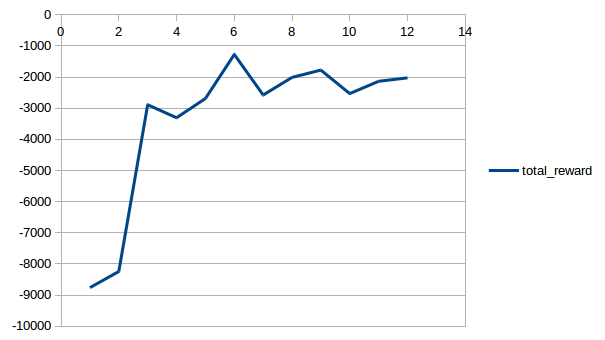
\includegraphics{images/hover.png}
\caption{Reward vs episodes plot for hover task}
\end{figure}

    \hypertarget{task-3-landing}{%
\subsection{Task 3: Landing}\label{task-3-landing}}

What goes up, must come down! But safely!

\hypertarget{implement-landing-agent}{%
\subsubsection{Implement landing agent}\label{implement-landing-agent}}

This time, you will need to edit the starting state of the quadcopter to
place it at a position above the ground (at least 10 units). And change
the reward function to make the agent learn to settle down
\emph{gently}. Again, create a new task for this (e.g. \texttt{Landing}
in \texttt{tasks/landing.py}), and implement the changes. Note that you
will have to modify the \texttt{reset()} method to return a position in
the air, perhaps with some upward velocity to mimic a recent takeoff.

Once you're satisfied with your task definition, create another agent or
repurpose an existing one to learn this task. This might be a good
chance to try out a different approach or algorithm.

\hypertarget{initial-condition-states-and-rewards}{%
\subsubsection{Initial condition, states and
rewards}\label{initial-condition-states-and-rewards}}

\textbf{Q}: How did you change the initial condition (starting state),
state representation and/or reward function? Please explain below what
worked best for you, and why you chose that scheme. Were you able to
build in a reward mechanism for landing gently?

\textbf{A}: I changed the starting state from (0,0,\textasciitilde{}0)
to (0,0,h). `h' is the height from which you want the quadcopter to
start landing. I also gave some initial vecocity of 10 at the z axis so
as to minimize the effect of gravity. The landing was not that gentle I
expected, but it was good enough after few episodes. Reward function I
used -

\begin{verbatim}
reward = -(abs(pose.position.z)*3 + abs(angular_velocity.x) + abs(angular_velocity.y) + abs(angular_velocity.z) + abs(linear_acceleration.x) + abs(linear_acceleration.y) + abs(linear_acceleration.z) + abs(pose.orientation.x) + abs(pose.orientation.y) + abs(pose.orientation.z)) # reward = zero for matching target z, -ve as you go farther

 #Normalized the reward
 reward = reward / 4
 if pose.position.z <= 0:  # agent has crossed the target height
    reward += 10.0  # bonus reward
    done = True
 elif timestamp > self.max_duration:
 reward -= 10.0  # extra penalty
    done = True
\end{verbatim}

I took terms of angular velocity,linear acceleration and pose into
account.

\hypertarget{implementation-notes}{%
\subsubsection{Implementation notes}\label{implementation-notes}}

\textbf{Q}: Discuss your implementation below briefly, using the same
questions as before to guide you.

\textbf{A}: I took terms of angular velocity,linear acceleration and
pose into account to build a reward function. And the policy I used was
general enough to scale to this task also.

\hypertarget{plot-episode-rewards}{%
\subsubsection{Plot episode rewards}\label{plot-episode-rewards}}

As I have general policy which can run in multiple scenario's. The only
task was to come up with a good reward function.
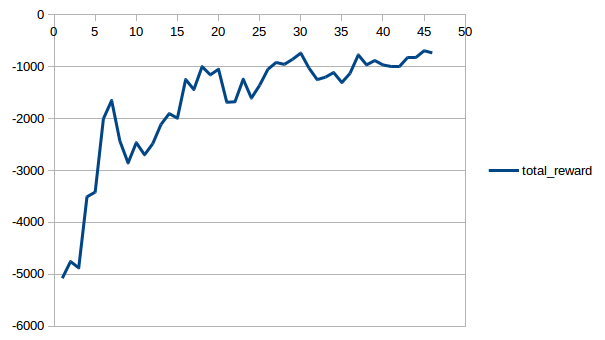
\includegraphics{images/landing.png}

    \hypertarget{task-4-combined}{%
\subsection{Task 4: Combined}\label{task-4-combined}}

In order to design a complete flying system, you will need to
incorporate all these basic behaviors into a single agent.

\hypertarget{setup-end-to-end-task}{%
\subsubsection{Setup end-to-end task}\label{setup-end-to-end-task}}

The end-to-end task we are considering here is simply to takeoff, hover
in-place for some duration, and then land. Time to create another task!
But think about how you might go about it. Should it be one meta-task
that activates appropriate sub-tasks, one at a time? Or would a single
combined task with something like waypoints be easier to implement?
There is no right or wrong way here - experiment and find out what works
best (and then come back to answer the following).

\textbf{Q}: What setup did you ultimately go with for this combined
task? Explain briefly.

\textbf{A}: Since the end-to-end task is open-ended. I used the same
policy and changed only reward function to perform the final task.I used
approaches to combine the rewards(takeoff,hover,landing) into one
general reward.

\hypertarget{implement-combined-agent}{%
\subsubsection{Implement combined
agent}\label{implement-combined-agent}}

Using your end-to-end task, implement the combined agent so that it
learns to takeoff (at least 10 units above ground), hover (again, at
least 10 units above ground), and gently come back to ground level.

\hypertarget{combination-scheme-and-implementation-notes}{%
\subsubsection{Combination scheme and implementation
notes}\label{combination-scheme-and-implementation-notes}}

Just like the task itself, it's up to you whether you want to train
three separate (sub-)agents, or a single agent for the complete
end-to-end task.

\textbf{Q}: What did you end up doing? What challenges did you face, and
how did you resolve them? Discuss any other implementation notes below.

\textbf{A}: For combinig the above 3 rewards into one generalized
reward.I used 2 approaches. - Normalizing all the 3 rewards and adding
them into one single reward. - Made reward function dynamic and
dependent on time. I used the earlier 3 rewards fuctions based on time.
For first 2sec - Takeoff reward, next 2sec- hover and at last landoff
reward. Seocnd approach performed better than the first one. But still
they didn't performed as expected. I also used the approach of
training/predicting only z-axis force and rest making them 0(this
knowledge I get from the problem domain), this approach gave very good
results. I feel that there should be clarification given to the student
wheter to use the problem domain knowledge or not in this project.
Whether to make the agent generalized or specific to these tasks only.

\hypertarget{plot-episode-rewards}{%
\subsubsection{Plot episode rewards}\label{plot-episode-rewards}}

\begin{figure}
\centering
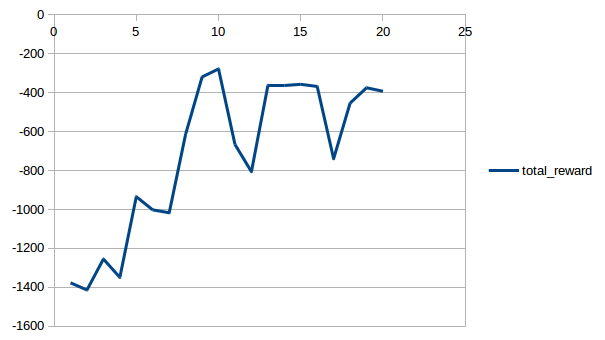
\includegraphics{images/all.png}
\caption{Reward vs episodes plot for end-to-end task}
\end{figure}

    \hypertarget{reflections}{%
\subsection{Reflections}\label{reflections}}

\textbf{Q}: Briefly summarize your experience working on this project.
You can use the following prompts for ideas.

\begin{itemize}
\tightlist
\item
  What was the hardest part of the project? (e.g.~getting started,
  running ROS, plotting, specific task, etc.)
\item
  How did you approach each task and choose an appropriate
  algorithm/implementation for it?
\item
  Did you find anything interesting in how the quadcopter or your agent
  behaved?
\end{itemize}

\textbf{A}: There was different chalenges at different steps. I enjoyed
working on this project a lot. Also I learned a lot and understood the
working of the ROS and its interactions with the simulator. I choose a
generic algorithm which catered all my beeds, I used Continuous control
with deep reinforcement learning(DDPG) algorithm to train the
quadcopter. Initially the quadcopter did not know what to do, how to
fly. But after few episodes it learnt what to do and how to fly.There
was a lot of toppling and spinning in the first case as there was not
any penalty in reward for not doing so. If we can include a penality
term in the first reward function then that will solve the problem of
toppling/spinning.

There are few feddback I want to provide - - Setting up the ROS - People
are facing some issues in setting up the ROS environment. I also faced
some but was able to resolve it. Here are my some thoughts which I get
form setting of the ROS environment. If we can put these into the README
then that can help the students in dubuggin. * Make sure that you can
ping the vm IP from the your Mac and Mac IP from vm.If the IP of vm is
a.b.c.d . Run the command ping a.b.c.d and see if packets are being sent
from both ways. * In the rossetting file. Make sure that both the flags
are true.

\begin{itemize}
\tightlist
\item
  As pointed out earlier, just by looking at the problem domain for take
  off, hover, landing we can deduce that only z-force plays the part.
  Rest all the parameters are not significant. So one can always do -

  \begin{itemize}
  \tightlist
  \item
    x-force = 0
  \item
    y-force = 0
  \item
    z-force = predict only this parameter by neural network.
  \item
    x-torque = 0
  \item
    y-torque = 0
  \item
    z-torque = 0
  \end{itemize}
\item
  Using this kind of neural network modelling one can ensure that the
  quadcopter does not topples and always move in z-direction.
\item
  In README there should be more clarification regarding this, is the
  student allowed to use the domain knowledge and train the quadcopter
  or he should train quadcopter in a general fashion. Should he train
  for all the 6 parameters or he can train 1 parameter and keep all
  other 0 ?
\end{itemize}


    % Add a bibliography block to the postdoc
    
    
    
    \end{document}
